
\chapter{Physical Layer Components}

In Chapter~\ref{ch:repeaters}, we saw the basics of a quantum repeater and how it can distribute entanglement over long distances. In this chapter, we will go a little bit deeper and see how individual physical components of a quantum repeater work.

\section{Introduction}

\begin{figure}[t]
    \centering
    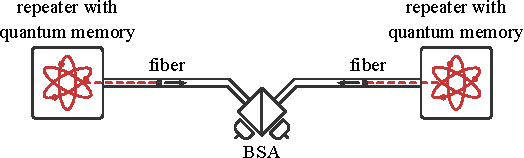
\includegraphics[width=0.7\textwidth]{lesson13/13-1_repeater.pdf}
    \caption[MIM link hardware]{An MIM link. The nodes at each end are repeaters with memories, shown by the atom symbols.  The node in the middle is the Bell-state analyzer (BSA).  The red circles represent photons in flight, entangled with the memories.}
    \label{fig:13-MIM-link}
\end{figure}


Fig.~\ref{fig:13-MIM-link} shows the basic architecture for a quantum repeater link. We have our network nodes, represented by the \rdv{blue boxes}, and they each have some qubits \rdv{represented by the atom symbols}.  They fire photons (\rdv{orange ovals}) toward the middle node, which we know implements a Bell-state measurement. That way, we can establish entanglement over long distances. But, what are the individual physical components of a quantum repeater system, and more importantly how can we implement them? First, we need optical fibers to carry our photons. That's kind of obvious, and already we have covered optical fibers at some length in Chapter~\ref{sec:7_waveguides}\index{optical fiber}. The next thing that we need is the Bell-state analyzer in the middle. The analyzer implements our Bell-state measurement, which is crucial for implementing entanglement swapping.

While the photons are in flight and traveling toward our Bell-state analyzer (BSA)\index{Bell-state analyzer (BSA)}, the qubits stored in the nodes are stationary. They are not moving anywhere, so we must have some physical means of storing these qubits, which we do with the help of \emph{quantum memory}\index{quantum memory}. The difference between classical memories and quantum memories is quite substantial. Classical memories are usually stored as zeros and ones, only classical bits, whereas quantum memories have to be able to store not only one or zero, but also any superposition, and in fact any entangled state. That way, they can share entanglement over the entire quantum network. After talking about the two basic components of BSAs and memories, we will consider how all of these components work together to implement a quantum repeater. Most importantly, we will also consider the various factors that affect the success rate of our quantum repeater and entanglement swapping scheme. So, we will spend the first half of this chapter talking about Bell-state analyzers. We will revisit measurements and how they can actually be implemented, and what it means to measure in different bases, and how can we implement different basis measurements with Pauli $Z$ measurements and some unitaries. Then, we will move on to the quantum circuit for a Bell-state measurement, and from that we will talk about real-world implementation of Bell-state measurements with linear optics.  In the latter half of this chapter we will talk about memories. We will begin with consideration of what a good quantum memory should be like, then we'll move on to the candidate systems.  We say "candidate" because at the moment, there is no leading physical system that is considered to be the best quantum memory. All of the existing candidate systems have some advantages and some drawbacks, which we will consider in the latter half of this chapter.



\section{Bell State Measurements I}

\rdv{this par needs work, but I haven't decided what to do with it. Do we really need to repeat the Bell states here?}
Let's remind ourselves what Bell states look like.  The Bell states are four entangled states, and they can be written in this form in the computational basis. \ket{\Phi^+} is a superposition of  \ket{00}, and  \ket{11}. So is \ket{\Phi^-}, but with a negative phase between the two, and this (follow pointer) is the expression for \ket{\Psi^+}, and \ket{\Psi^-}. We saw that these states are orthonormal. This means that if you take the inner product of a Bell state with itself, for example, \ket{\Phi^+}, then you get a one, which means that it is normalized. But if you take an inner product of one of the Bell states with a different Bell state, then you get a zero. For example, the inner product between \ket{\Phi^-} and \ket{\Phi^+} is zero, and so on,
\begin{equation}
\begin{aligned}
&\left\langle\Phi^{+} \mid \Phi^{+}\right\rangle=1 \\
&\left\langle\Phi^{-} \mid \Phi^{+}\right\rangle=0.
\end{aligned}
\end{equation}

Since the Bell states are orthonormal and completely cover the possible space of two qubits, we can take any pure state of two qubits, and write it out in terms of Bell states, which we call writing it in the Bell basis\index{Bell basis}. For example, let's consider a general pure two-qubit state in the computational basis with probability amplitudes given by $\alpha$, $\beta$, $\gamma$, and $\delta$,
\begin{equation}
|\psi\rangle=\alpha|00\rangle+\beta|01\rangle+\gamma|10\rangle+\delta|11\rangle.
\end{equation}

Back in Ch.~\ref{sec:8-2_teleportation_protocol}, in the context of teleportation, we saw how to rewrite the computational basis states \ket{00}, \ket{01}, \ket{10} and \ket{11} in the Bell basis. Now we have a general two-qubit state, which is of course a superposition of the four Bell states, where naturally the probability amplitudes have changed. For example, the probability amplitude for state \ket{\Phi^+} is $(\alpha+\beta)/\sqrt{2}$, and so on for the other Bell states,
\begin{equation}
|\psi\rangle=\frac{\alpha+\beta}{\sqrt{2}}\left|\Phi^{+}\right\rangle+\frac{\alpha-\beta}{\sqrt{2}}\left|\Phi^{-}\right\rangle+\frac{\gamma+\delta}{\sqrt{2}}\left|\Psi^{+}\right\rangle+\frac{\gamma-\delta}{\sqrt{2}}\left|\Psi^{-}\right\rangle
\end{equation}

We have been treating measurements as a question that we ask about the state of our physical system, and the question in this case is, which of the four Bell states is our state in? Is it the state \ket{\Phi^+}? Is it the state \ket{\Phi^-}, \ket{\Psi^+}, or \ket{\Psi^-}? This is what the measurement reveals about our system, and usually we say that we get the answer with some probability. For example, depending on the initial state \ket{\psi}, we might get the answer that the state is \ket{\Phi^+}. In this case, that answer would occur with a probability which is the modulus squared of the original complex probability amplitude,
\begin{equation}
\operatorname{Prob}\{\ket{\Phi^+}\}=\left|\frac{\alpha+\beta}{\sqrt{2}}\right|^2.
\end{equation}
This is a very abstract notion of what a measurement actually is, and it's not very useful when it comes to doing calculations. Shortly, we will see how to actually implement such a measurement in terms of a quantum circuit, which will tell us more about what these measurements are actually doing and how we can implement them in a laboratory.

Before we do that, let's step back a little bit and consider something simpler. Let's look at measurement of a single qubit, and let's be specific and say that we want to measure the single qubit in the Pauli $Z$ basis.

\rdv{simple figs here with the measurement symbols for Z, X, and H+Z measurement. accompanying text needs cleanup.}

In the quantum circuit notation, we would write it as this: we have some input state \ket{\psi}, and then we measure it- this is the symbol for measurement (see figure), and here, this little Z is just reminding us that we are measuring in the $Z$ basis.  So, what we get is that initially, if the state is some general superposition of \ket{0} and \ket{1} with probability amplitudes $\alpha$ and $\beta$, then the measurement can give us a $+1$ outcome with corresponding probability, which is given by the inner product between the initial state and our basis state \ket{0} modulus squared, which is just $\alpha$ modulus squared. Or, we can get the  $-1$ outcome which is given by the probability given by $\beta$ modulus squared, the probability amplitude of the basis state one.

Now, let's try to do a measurement in the $X$ basis.

Again, in the quantum circuit notation, it would look like this: we have our initial state \ket{\psi}, and we're doing a measurement, and now it's in the $X$ basis which is over here (see figure) written by this little X.  (If you see this symbol in a circuit without the Z or X, generally this means to measure in Z basis.) Again, we are considering some general input state, but in order to be able to determine the probabilities of the different outcomes, we are going to rewrite this state in the $X$ basis. So we have seen that \ket{0} is equal superposition of the \ket{+} state and the \ket{-} state, and similarly one is an equal superposition as well, but this time we have a negative phase between \ket{+} and \ket{-} states. So, we can rewrite the initial state in this following form (see pointer, RHS eq), and from this form we can easily read out the probabilities of obtaining the  $+1$ outcome of the measurement, which is given by half $\alpha$ plus $\beta$, the whole thing modulus squared, and the probability for the  $-1$ outcome.

But now, let's impose a restriction on ourselves. Let's say that we cannot perform measurement in the $X$ basis. Let's say we're only allowed to do measurements in the $Z$ basis, what do we do then? Well, we can consider the following quantum circuit: we have the initial state and then we do some unitary operation on that state. Here (see figure), we are choosing the Hadamard, and then we perform our measurement but this time in the $Z$ basis.

\rdv{from here to the end of the section needs cleanup.}

So, we start with the usual initial state, it's a superposition of \ket{0} and \ket{1}, but then after application of the Hadamard gate we get a new state, which we are denoting \ket{\psi'}, and this new state is given in this form (follow pointer). Just to remind you, Hadamard, when it's applied on \ket{0}, gives us a \ket{+} state, so an equal superposition of \ket{0} and \ket{1}, whereas Hadamard applied to one gives us the \ket{-} state, and then if we just expand the \ket{+} state and the \ket{-} state again in the computational basis, we arrive at this form for our state \ket{\Psi^+}. And now, because we are doing measurement in the $Z$ basis, again it's easy to read out the probabilities corresponding to outcomes $+1$ and $-1$.

But look, even though here we have a different quantum circuit, we are obtaining the outcomes $+1$ and $-1$ with the same probabilities as we had done on the previous slide. So, what this shows is that there are two ways of implementing a Pauli $X$ measurement. We can do it directly, writing it like this, or if we want we can just measure in the $Z$ basis, but then we have to apply some unitary transformation on our pure state \ket{\psi}.

So, why is that? Well, the clue is in the probabilities. If you look at the probability of the $+1$ outcome in this scheme (see pointer), where we are measuring the $X$ basis directly, then it's given by the inner product of \ket{\psi} and the \ket{+} state modulus squared. If we do it in our other scheme where we are using the Hadamard followed by a z-measurement, then it's given by the corresponding expression here (see pointer), now it's the inner product between the state \ket{\psi'}, so this is our initial state after we apply Hadamard to it, and the inner product is with a \ket{0} state.

And then, what we get is \ket{\psi} times Hadamard times \ket{0}. So what we are getting is, really, if we are comparing these two probabilities (follow pointer), we see that this \ket{\psi} state has an inner product with \ket{+}, and \ket{+} is just written as Hadamard applied to a \ket{0} state. So that's what we are doing here (top right red box circuit).

So what we are really doing is we are asking: what unitary takes me from a \ket{+} state to a \ket{0} state, or from a \ket{0} state to a \ket{+} state? And we already know this unitary, it's the Hadamard. Similarly for the  $-1$ outcome, we look at the different probabilities and what we get is, again, we go from a \ket{-} state to a \ket{1} state via the Hadamard transformation.

So the Hadamard transforms our desired basis of measurement, which in this case is a Pauli $X$ into a Pauli $Z$ basis.

Now, how to do a Bell measurement using only Pauli $Z$? Well, we have two qubits, so we're going to need two Pauli measurements, and we are going to need to apply some two-qubit unitary before we actually measure the state. So the question now is, how do we find this unitary?

Well, we know one thing that the unitary when applied to a state \ket{\Psi^+} should give us a \ket{00}. When applied to state \ket{\Phi^-}, it should give us state \ket{10}, and so on and so forth. So this is our rule of transforming from our Bell-basis into our computational basis, and if we can do that, then we can just measure in the $Z$ basis. In the same way we saw how it worked for the Pauli $X$ basis, we had to find a unitary that transforms from the $X$ basis into the $Z$ basis which was given by Hadamard. Here, we are looking for a more general unitary because it's acting on two qubits.

So, without further ado, this is the circuit that actually achieves our desired transformation (fig. on slide). It's given by a CNOT gate, which is given by this two qubit gate, followed by a Hadamard on the first qubit, and then two measurements in the $Z$ basis. And what happens, that if we get outcomes \ket{00}, which corresponds to  $+1$  $+1$ \rdv{how should we format this?}, then we know that we have a Bell-state \ket{\Phi^+}, and similarly for all the other three possible measurement outcomes, and each individual measurement outcome represents uniquely a Bell-state measurement.

So, this is true in general, that any measurement basis can be implemented by Pauli $Z$ measurements and a suitable unitary applied before we measure our qubits.

And this trick is very useful, particularly in quantum computation, and also in quantum communication, and in the next step we will actually see how we can do this in real life using linear optics.



\section{Bell State Measurements II}
\label{sec:13-3_Bell_state_measurement_2}

In this section, we will talk about how to actually implement a Bell-state measurement with linear optics. The actual scheme really depends on our encoding. So let's just pick some encoding for our qubits, for example linearly polarized single photons. There are two reasons for this choice: one, it's intuitive and simple so it makes a good pedagogical example, and two, it's one of the most commonly used encodings in real experiments.

In this encoding, we encode our qubit in a state \ket{0} as a single photon that's polarized in the vertical direction, which we write as \ket{V}. Our other computational basis state \ket{1}, as a single photon polarized in the horizontal direction, we write \ket{H}.

\begin{figure}[t]
    \centering
    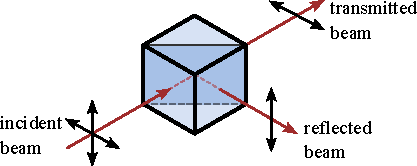
\includegraphics[width=0.6\textwidth]{lesson13/13-3_PBS.pdf}
    \caption[A polarizing beam splitter (PBS)]{The action of a polarizing beam splitter (PBS).  The vertical rays represent vertically polarized light \ket{V}, while the diagonal rays represent horizontally polarized light \ket{H}.  The direction of propagation, red arrows, is normal to the \ket{H}-\ket{V} plane.}
    \label{fig:13-PBS}
\end{figure}


% \rdv{Make Figs. X.a, X.b, c and d from p. 21-24}

The first question that we should ask is, "how do we implement a Pauli $Z$ measurement with this encoding"? Well, we have to measure and distinguish the two different polarizations, horizontal and vertical. That can be done with a little piece of crystal called a \emph{polarizing beam splitter} (PBS)\index{polarizing beam splitter (PBS)}, as shown in Fig.~\ref{fig:13-PBS}. If you have a beam of light coming in with some polarization, a PBS splits the beam of light into two beams. One is transmitted through the polarizing beam splitter but comes out only with a horizontal polarization, while the other one gets reflected by the PBS and is polarized in the vertical direction. (The relative strength of the two beams naturally depends on the polarization of the input light.)
Thinking in terms of computational states, we now have two beams, one for our \ket{0} and one for our \ket{1}.

\begin{figure}[t]
    \centering
    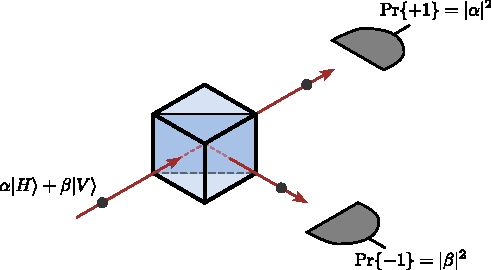
\includegraphics[width=0.7\textwidth]{lesson13/13-3_PBS_measure.pdf}
    \caption[A polarizing beam splitter (PBS) measuring a qubit]{A PBS measuring an arbitrary photonic qubit in the \{$|H\rangle$, $|V\rangle$\} basis.}
    \label{fig:13-PBS-measure}
\end{figure}

Assume that we have a single photon polarized in the vertical direction, and we place two detectors after the polarizing beam splitter to detect which output path was taken by the single photon. If the photon is horizontally polarized, it gets transmitted through the polarizing beam splitter.
Therefore, it gets detected by the detector placed in the transmitted path with probability one.
This represents our measurement outcome of $+1$.
It never happens that a vertically polarized photon gets transmitted, therefore the detector placed in the reflected path never gets triggered.
The probability of the outcome $-1$ is 0.
On the other hand, if the initial photon is vertically polarized, it always gets reflected and travels down into the bottom detector, where it always gets detected.
The probability of the outcome $-1$ is 1, and the probability of the outcome $+1$ is always 0.

Now, what happens if we put in a superposition of these two linear polarizations, as in Fig.~\ref{fig:13-PBS-measure}?
Our input state is given by $\alpha\ket{H} + \beta \ket{V}$.
The photon has a chance to get transmitted, with probability given by $|\alpha|^2$, and it also has a chance to get reflected and travel down into the other detector corresponding to the measurement outcome $-1$ (bottom), with probability of $|\beta|^2$.
This implements a $Z$ measurement.
We have seen in the previous step that for a Bell-state measurement, we need two measurements in the $Z$ basis and a suitable unitary.
Let's see what happens when we take two sub-units like the one in Fig.~\ref{fig:13-PBS-measure} and join them with a regular (not polarizing) fifty-fifty beam splitter, as in Fig.~\ref{fig:13-BSA-clicks}. Assume we have two photons, one coming from the top and one coming from the left, and they arrive at the beam splitter at the same time.
A complete analysis would require a little bit more quantum optics than we have studied so far, so instead of the full derivation, here we will give you the result. Depending on which of the four detectors click, we may learn which Bell-state has been measured. Let's see what the different patterns are.

\begin{figure}[t]
    \centering
    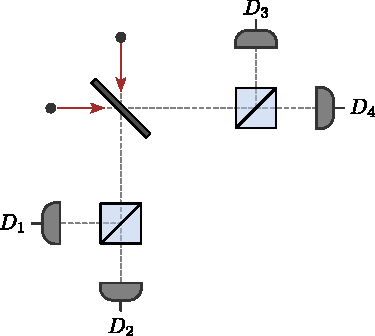
\includegraphics[width=0.6\textwidth]{lesson13/13-3_BSA_clicks.pdf}
    \caption[A four-detector Bell-state analyzer (BSA)]{A BSA measuring a pair of qubits, one arriving at the initial beam splitter from above and one from the left.  Different click patterns on the four detectors may confirm projection into a Bell state, or be ambiguous.}
    \label{fig:13-BSA-clicks}
\end{figure}

If we get a joint detection in detectors D1 and D4, meaning that both of these detectors click, then we have implemented a successful Bell measurement, and the outcome corresponds to the projection onto the state \ket{\Psi^-}. Also, if we get a joint detection in D2 and D3, then we can also say that we have implemented a successful Bell measurement, and the result corresponds to the state \ket{\Psi^-}. A different pattern of detection that we can get is a joint detection at the two detectors in the lower branch of our Bell-state analyzer, so if both D1 and D2 click, then we can conclude that we have a state \ket{\Psi^+}, so this corresponds to another successful Bell measurement. Equally, if we get both detectors clicking in the right branch of our Bell-state analyzer, so if both D3 and D4 click, then we can also conclude that we have a Bell-state \ket{\Psi^+}.

It is also possible that both photons travel into a single detector. All four detectors are equally probable. However, because more than one Bell state can result in this happening, the answer we get is ambiguous. We cannot say that whether we have \ket{\Phi^+} or \ket{\Phi^-}.
%So whenever we get only one of these detectors triggered, then we know that we have one of the state \ket{\Psi^+} or \ket{\Psi^-}, but we cannot tell which one. 
This is a bit of a problem because we cannot fully implement a Bell-state measurement. We cannot distinguish all four Bell states, only two of them, \ket{\Psi^+} and \ket{\Psi^-}.

\begin{table}
\centering
\begin{tabular}{p{0.55in}|c|p{1.5in}|c}
pattern  & result & reason & action \\\hline
D1 and D4 & \ket{\Psi^-} & & keep and use \\
D2 and D3 & \ket{\Psi^-} & & keep and use \\
D1 and D2 & \ket{\Psi^+} & & keep and use \\
D3 and D4 & \ket{\Psi^+} & & keep and use \\
any single click & \ket{\Phi^\pm} (amb.)  & two photons together, or only one arrived & discard \\
no click & (N/A) & photons lost, detection failure & discard \\
any other pattern & (N/A) & detection error & discard
\end{tabular}
\caption{4-detector BSA click patterns and their outcomes. amb., ambiguous}
\label{tab:bsa-clicks}
\end{table}

\rdv{added some discussion of loss}
This means that a complete, unambiguous Bell-state measurement cannot always be successfully implemented with linear optics. In fact, even with 100\% probability of receiving both photons, the maximum probability of a successful Bell measurement is limited to only 50\%.  Of course, as we saw when discussing the loss of photons in fiber, the loss of one or both photons is highly probable, increasing the ambiguity of interpreting the result of one click.  These cases (along with the case where something goes wrong in the hardware) are summarized in Tab.~\ref{tab:bsa-clicks}. 
%We have seen in a previous chapter that quantum repeaters have to contend with a lot of noise. To deal with that noise, we have to purify our states. We have also seen in previous chapters that we have to deal with lossy fibers, which was the original motivation to develop quantum repeaters. But even if we take away all of these sources of error, there is still a fundamental error in the fact that Bell-state measurement cannot be always successfully executed with linear optics. 
On top of that, we have to take into account that the two photons coming into our Bell-state analyzer have to be synchronized. If they come in close enough together that two detectors click almost simultaneously, but not close enough together to be indistinguishable, we may misinterpret the result. The Bell-state measurement has failed and we did not establish entanglement between the network nodes, but may not realize it; when we accumulate statistics about the link, this results in lowered fidelity.


\section{Stationary and flying qubits}

First, let's begin talking about what factors matter -- what does a good memory look like, and what requirements should it satisfy?  We will start with the \emph{DiVincenzo criteria}\index{DiVincenzo criteria}. These criteria were introduced in the context of quantum computation, but they also apply in the context of quantum networking, with slightly different emphasis on which ones are important.  The extended list of these criteria, with five for quantum computing and two more for quantum communication, is:

\begin{enumerate}
    \item Well-defined qubit
    \item Can be initialized
    \item Long lifetime
    \item Universal gate set
    \item Efficient measurement
%For communications, we also want:
    \item Convert or entangle stationary \& flying qubits
    \item Able to carry flying qubits long distances
\end{enumerate}

First, if you want to build a good quantum computer, you need a well-defined qubit. Now, qubits don't come for free in nature. Usually, we have very complicated systems with many different energy levels. In order to have a good well-defined qubit, you must be able to take a system for which you can address two of those energy levels, distinguish them and control them as a pair, without slipping into the other energy levels.  (Sometimes a third level is used as a temporary state to achieve certain effects such as emitting a photon, but the computation is done by restricting your actions to the two levels we want to use.)

Second, you need to be able to initialize this qubit. Initialization is important because then you know exactly from what state your quantum computation can start, so if you have a good procedure for initializing your qubit, that allows you to also carry out good quantum computation.  (This also sometimes involves the temporary use of a third state.)

Third, you want long lifetimes, meaning that when you put your qubits in a superposition of states, they don't decohere very quickly. Long lifetimes allow you to carry out longer and longer quantum computations, which of course you need if you want to solve harder and harder problems.  This criterion is especially important in quantum networking, as we will see below.

Fourth, you must be able to implement a universal set of gates. Your qubit and your physical system typically have a couple of ways that the bit can be manipulated, with a parameter for how long you turn on the effect.  This set needs to be designed such that they can collectively produce an arbitrary unitary evolution. If you can rotate any point on the Bloch sphere to any other point and you can entangle two qubits, that is enough.

Fifth, of course, we need efficient measurements. Just carrying out transformations of the state in a quantum manner is not enough, you somehow have to extract the information at the end of the quantum computation.

In the context of quantum communication, we have two more requirements to consider. The first of these is conversion or entanglement between stationary and flying qubits, which we already saw earlier in this chapter. Stationary qubits are those qubits that are sitting in our quantum network nodes, loaded into the quantum memories.
%They don't really move, which is why we call them stationary. 
Flying qubits are those qubits that are used for entanglement swapping in the BSAs to create link level entanglement between between the quantum memories. We must be able to entangle photons (the flying qubits) with the stationary qubits inside the memories, but also we must be able to use entanglement swapping to create end-to-end entanglement.

Lastly, we also must be able to transport flying qubits over long distances.

Here, we will look at memory lifetime and the two communications requirements.

Why is memory lifetime important? In computers, if our memory lifetime is long, and also our gate speeds are fast, we are able to implement longer, more complex computations.  Thus, the ratio of gate speed to memory lifetime is an important factor. In the context of quantum communication, we often store qubits for long periods of time without acting on them, as we await messages from partners in the network.  Therefore, what's really important is not the gate speed itself, but the ratio of memory lifetime to communication time, 
provided that the gate time is short compared to the round trip time (RTT). Let's consider how we establish link level entanglement. We start with quantum memories, and they emit photons. These photons are entangled with the memories, and they travel, let's say to a Bell state analyzer that is halfway between the quantum nodes. There, we perform a Bell-state measurement, but then we also have to communicate classically back to the nodes about the outcome of the Bell-state measurements, and this is our node-to-BSA round trip time~\footnote{RTT for a link can be node to BSA and back again in some contexts, or all the way memory node to memory node and back again in others. It should be clear from the context which we mean.}. If our memory lifetime is shorter than the RTT, then we cannot really do much. Even if we successfully perform the Bell-state measurements on those photon pairs, by the time the return messages are received, our memories decohere and are not useful anymore.

To give you some idea of the latency values that we're talking about, see Tab.~\ref{tab:rtt}. The speed of light in a fiber is approximately $0.2$ meters per nanosecond,
%two hundred millimeters per nanosecond, 
so if our nodes are one kilometer apart, one round trip from one node to the other and back takes ten microseconds. For a hundred kilometers, it increases to one millisecond, and for ten thousand kilometers it goes all the way up to a hundred milliseconds (0.1 seconds) per round trip time.  The values \emph{five nanoseconds per meter one way} and \emph{10 microseconds per km round trip} are easy metrics to remember.

\begin{table}
\centering
\begin{tabular}{l|r}
distance (km)  & RTT in fiber \\\hline
1     & $10\mu$sec \\
10    & $100\mu$sec \\
100   & $1$msec \\
1,000 & $10$msec \\
10,000 & $100$msec
\end{tabular}
\caption{Round trip times in optical fiber.}
\label{tab:rtt}
\end{table}

Now, what are the processes that are degrading our memories? The two main processes are \emph{energy relaxation}\index{energy relaxation} and \emph{dephasing}\index{dephasing}, and they are characterized by two different time scales, referred to as the $T_1$ time\index{$T_1$ time} scale and the $T_2$ time\index{$T_2$ time} scale.  $T_1$ characterizes the energy relaxation time, whereas $T_2$ gives us the characteristic dephasing time. First, let's consider the energy relaxation time given by $T_1$.

\begin{equation}
\begin{aligned}
&T_1:|1\rangle \rightarrow|0\rangle \\
&\operatorname{Prob}(\ket{1})=e^{-t / T_1}
\end{aligned}
\end{equation}

This basically tells us how quickly our qubit decays from the excited state to the ground state, or from state \ket{1} into state \ket{0}. If we initialize our state in \ket{1}, the probability that after some time $t$ we still find it in the state \ket{1} is given by the expression $e^{-t/T_1}$. The probability that after $T_1$ seconds we still find our state in \ket{1} is given by $\frac{1}{e}$. This process of going from \ket{1} to \ket{0} captures the fact that usually \ket{1} is encoded into a state of our quantum memory that has a higher energy, while \ket{0} in a lower-energy state such as the ground state, although of course that choice is by convention, not an immutable fact of physics.  That's why we call $T_1$ the energy relaxation time.

The dephasing time gives us the time scale for the loss of phase coherence in our qubit. If we are only use qubits to implement classical communication,  $T_1$ is important but  $T_2$ not so much, because there is no quantum coherence and we are not using superpositions. But in quantum networking and quantum communication, superpositions are crucial, and those superpositions can be destroyed by this dephasing process.

If we start in an equal superposition of \ket{0} and \ket{1} (the \ket{+} state), $T_1$ is the characteristic time scale that tells us when we will end in a completely mixed state,
\begin{equation}
\begin{aligned}
\rho_{\textrm{completely mixed}} =\frac{\ketbra{0}{0}+\ketbra{1}{1}}{2}.
\end{aligned}
\end{equation}
In Sec.~\ref{sec:3-3_density_matrices}, we saw the crucial difference between complete mixtures and equal superpositions. Here, if we prepare the state in the pure state, after some time $t$ we will have the mixed state
% $T_2:|+\rangle \rightarrow$ completely mixed state
\begin{equation}
\begin{aligned}
\rho=P|+\rangle\langle+|+\left(\frac{1-P}{2}\right)(|0\rangle\langle 0|+| 1\rangle\langle 1|)\text{, where }  P=e^{-t / T_2}.
\end{aligned}
\end{equation}
With probability $P$, we will still be in the ideal initial state, and with probability $1-P$, we will have decohered into a completely mixed state. Both of these processes, the relaxation process and the dephasing process, are \index{Poisson processes}\index{Poisson process}. It's a little bit ironic since we're talking about memories, but these processes are also called \emph{memoryless decay processes}\index{memoryless decay process}, meaning that their past history doesn't matter, only their current state.

We talked about the lifetimes of memories and why they are important, and we gave you some characteristic time scales which are very important when you are talking about communication over longer distances. Now, let's address the question of how we actually entangle atoms and photons.

\begin{figure}[t]
    \centering
    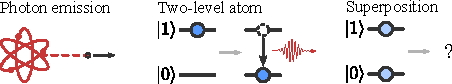
\includegraphics[width=0.7\textwidth]{lesson13/13-4_memory-first.pdf}
    \caption[First idea for memory]{Our first idea for a memory qubit is to use two energy levels of a system, such as ground and excited states of an atom.}
    \label{fig:13-memory-first}
\end{figure}

First, where is our qubit \ket{0} and \ket{1} in our quantum memory? Our quantum memory is a two level system for now, and it has a ground state \ket{g}, and some excited state of higher energy which we can label \ket{e}. These are natural candidates for representing \ket{0} and \ket{1}. For example, Fig.~\ref{fig:13-memory-first} shows a two level atom where $\ket{0}\equiv\ket{g}$ and $\ket{1}\equiv\ket{e}$. Now, how do we represent the flying qubit so that it works well with this memory qubit definition? One possibility is to use the presence or absence of a photon as a qubit, giving the definitions $\ket{0}\equiv\ket{\textrm{no photon},\ket{1}\equiv\ket{\textrm{photon}}}$.
We can see that if the atom decays from the excited state into its ground state, that is, it makes a transition from \ket{1} to \ket{0}, it emits a photon.

%\rdv{layout here isn't quite right, words in the middle should really be grouped with equations on the left}
\begin{equation}
\begin{array}{ll}
\text{memory qubit} & \text{flying qubit} \\

|0\rangle \equiv|g\rangle \quad \text { ground state } & \quad|0\rangle \equiv \mid \text {no photon}\rangle \\
|1\rangle \equiv|e\rangle \quad \text { excited state } & \quad|1\rangle \equiv \mid \text {photon}\rangle \\
\end{array}
\end{equation}

Now, how about coherences and superpositions? Well, we can prepare our memory in a superposition of the ground state and the excited state by applying an appropriately timed energy pulse, and our question is, "Well, what happens to the photon? Does it get emitted, or does it not get emitted? If it does get emitted, in what state will it be?" We see that the atom has a 50\% probability to be found in the ground state, where it cannot emit any energy, so our photonic qubit will be in the no photon, or \ket{0}, state. It also has a 50\% probability of being in the excited state, from where it can emit a photon. So in this way, we can think about our photonic qubit as being in a superposition of \ket{0} and \ket{1}, or \ket{\textrm{no photon}} and \ket{\textrm{photon}}.
This technique transfers the state \ket{+} from the atomic memory to the flying qubit and leaves the memory qubit in \ket{0}. 

% \begin{figure}[t]
%     \centering
%     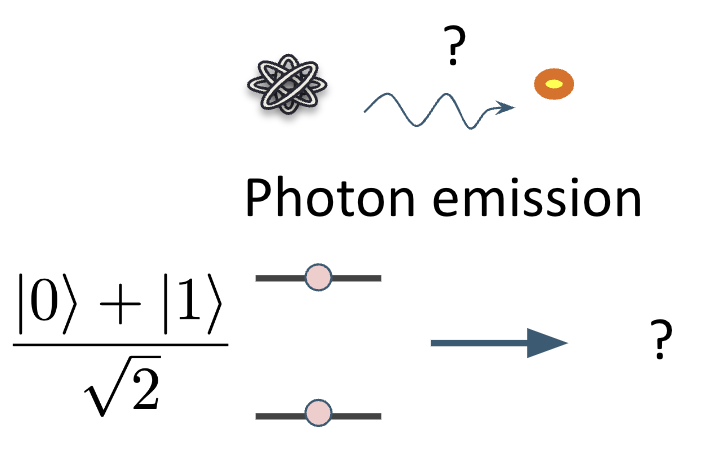
\includegraphics[width=0.7\textwidth]{lesson13/memory-first-idea-problem.png}
%     \caption[Problem with our first idea for memory]{Our first idea for a memory qubit appears to have a clean correspondence with the flying qubit, but then loss of the photon can make the state ambiguous.}
%     \label{fig:13-memory-first-problem}
% \end{figure}

\begin{figure}[t]
    \centering
    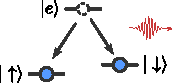
\includegraphics[width=0.3\textwidth]{lesson13/13-4_memory-second.pdf}
    \caption[Our second idea for memory]{Our second idea for a memory qubit is to use the post-decay spin of an atom. This allows us to use a polarized photon as a flying qubit robust against loss.}
    \label{fig:13-memory-second-idea}
\end{figure}

This is a very naive picture that demonstrates only some of the basic principles of how stationary and flying qubits interact. In real systems, things are a lot more complicated. In particular, when we look at this encoding of just having two levels for our quantum memory, it is usable but it's not a very good qubit. Due to the energy relaxation process, our excited state will eventually decay into a \ket{0}, destroying whatever message- whatever state we have encoded into the quantum memory. Similarly, our choice encoding for the flying qubit is not very good due to the attenuation of light in fiber. We described it in some detail that as we send photons down a fiber, attenuation means they are very likely to be lost. So, if we are waiting for some message at the end of the fiber and we don't receive a photon, we cannot be sure if the original message was really \ket{\textrm{no photon}} (\ket{0}), or if the initial message was \ket{\textrm{photon}} (\ket{1}) and the photon just got lost along the way. So, we have to be a little bit more careful and think how to encode our information in a better, more robust way.

What's our next choice for stationary memory qubit and flying qubit?

Consider the following atomic structure: we have two degenerate~\footnote{Meaning "having the same energy"; no moral weakness implied.} ground states, and we will label them as ground state up (\ket{\uparrow}) and ground state down (\ket{\downarrow}), as shown in Fig.~\ref{fig:13-memory-second-idea}. These can represent the two spins\index{spin} of our atom.
For our flying qubits, the matching state will be polarization, where \ket{0} will be represented by vertical polarization (\ket{V}), and \ket{1} will be represented by horizontal polarization (\ket{H}). 

% \rdv{layout here isn't quite right, words in the middle should really be grouped with equations on the left}
\begin{equation}
\begin{array}{ll}
\text{memory qubit} & \text{flying qubit} \\
|0\rangle \equiv|\uparrow\rangle \text { spin up } & |0\rangle \equiv|V\rangle \\
|1\rangle \equiv|\downarrow\rangle \text { spin down } & |1\rangle \equiv|H\rangle
\end{array}
\end{equation}

We prepare our atom initially in the excited state, and then the atom can decay, either to the ground state with spin up, or to the ground state with spin down, each with 50\% probability.  If the atom decays into the spin up state, the emitted photon will be vertically polarized.  If the atom decays into the spin down state, the photon will be horizontally polarized.  The thing is, we can only see that a photon comes out, and we don't actually know into which ground state the atom decayed. So, we are effectively implementing the following transformation: we go from the excited state of the atom to a superposition of the atom being found in the spin up state and the spin down state. 
%If that's true, then the photon that gets emitted just happens to have a vertical polarization. On the other hand, if it decays into the other ground state given by spin down, then the photon will have a horizontal polarization. So really, what we are doing is we are obtaining the following superposition of two qubits (top right eq.). 
Moreover, since the emitted photon depends on the final state of the atom, we now have an equal superposition of the atom being in the spin up state and the emitted photon being vertically polarized, and the atom being found in the spin down state and the photon being horizontally polarized. We can write this transformation as
\begin{equation}
\ket{e} \rightarrow \frac{\ket{\uparrow V}+\ket{\downarrow H}}{\sqrt{2}}
\end{equation}
where the arrows represent the post-decay state of the atom and the letters represent the polarization of the emitted photon.  (The left hand side of the equation has no photon, only the state of the atom.) In this way, we are entangling the flying photon with the stationary qubit of the memory.

Fig.~\ref{fig:13-MIM-energy} brings this all back to a concrete representation of our Bell-state analyzer. We have drawn this before very abstractly, but now we have a much better idea how it actually works in practice. In the middle are the two single mode fibers and on the left the two quantum memories at our two repeater nodes, separated by some distance, represented by their energy level diagrams. Each memory is prepared initially in the excited state \ket{e}, which decays into one of its ground states, either spin up \ket{\uparrow} or spin down \ket{\downarrow}. We don't know which state it decays into, leaving us with a flying photon that is entangled with its respective memory. These flying photons travel through the single mode fibers, then hit the central beam splitter, where (if all goes well) they interfere and we perform a Bell-state measurement using the other two beam splitters and the four detectors. In this way, we can establish link-level entanglement between the atomic memories sitting at the ends of the link. This is exactly the scheme that we have described previously for a midpoint-interference-memory (MIM) link, which in terms of physics is the same as a direct memory-to-memory connection (MM).

\begin{figure}[t]
    \centering
    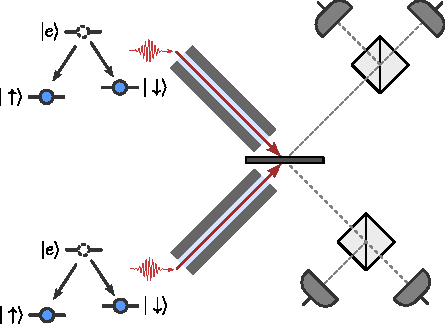
\includegraphics[width=0.7\textwidth]{lesson13/13-4_MIM_with_energy_levels.pdf}
    \caption[MIM with energy levels]{A different view of an MIM link. On the left are the energy level diagrams for the qubits, which decay into a superposition of two states while emitting photons entangled with the memories. On the right is a large view of the Bell state analyzer with three beam splitters and four photon detectors.}
    \label{fig:13-MIM-energy}
\end{figure}




\newpage
\begin{exercises}
\exer{Consider the following quantum state:}
\begin{equation*}
\ket{\psi} = \frac{\sqrt{3}}{2}\ket{0} + \frac{1}{2}\ket{1}
\end{equation*}
\subexer{Find the probability of measuring a zero.}
\subexer{Find the probability of measuring a one.}


\end{exercises}

\newpage
\section*{Quiz}
  \addcontentsline{toc}{section}{Quiz}

%\section{Learning more}

\section*{Further reading chapters 11-13}
  \addcontentsline{toc}{section}{Further reading chapters 11-13}

chapter 11

For those of you interested in how submarine fiber optic cables are made, laid and operated we recommend the following online article found here.\rdv{where???}

Our discussion of mode dispersion closely followed Section 5.6 of Hecht’s textbook and we encourage you to read it for the extra details that can be found in the book.

Qualitative review of classical amplifiers (with just the right amount of technical detail) can be here:

Emmanuel Desurvire, The Golden Age of Optical Fiber Amplifiers, Physics Today 47, 20 (1994).

Unfortunately this article is behind a paywall so you will have to use your university’s online system to access it.

chapter 12

Quantum repeaters are the "bread and butter" of quantum networks. A great place to learn more is here:

Rodney Van Meter, Quantum Networking, Wiley-ISTE, 2014.

Those of you interested in the paper that introduced the idea of a quantum repeater (and are not scared off by maths) might have a look here:

Hans J. Briegel, Wolfgang Dür, Juan I. Cirac, Peter Zoller, Quantum repeaters: The role of imperfect local operations in quantum communication, Physical Review Letters 81, 5932, 1998.

The paper is behind a paywall and needs to be accessed through your university’s library online services. An earlier version of the paper can be accessed openly here.

chapter 13

Great popular article about the physical layer components of quantum networks can be found here:
Dan Hurley, The quantum internet will blow your mind. Here’s what it will look like, Discover Magazine, 2020.

Another fantastic review of physical layer components can be found here:

Nicolas Sangouard, Christoph Simon, Hugues de Riedmatten, Nicolas Gisin, Quantum repeaters based on atomic ensembles and linear optics, Review of Modern Physics 83, 33, 2011.

Again, the published version is behind a paywall but the pre-publication version can be accessed for free here. Be warned though, this paper starts with an excellent introduction but the technical details ramps up quickly after that and relies on good grasp of quantum optics. So if you get lost after the introduction, don’t worry. You can come back to those parts later.
